\documentclass[10pt]{book}
\usepackage[utf8]{inputenc}
\usepackage[italian]{babel}
\usepackage{multicol}
\usepackage[bookmarks]{hyperref}
\usepackage[a4paper, total={18cm, 25cm}]{geometry}
\usepackage{listings}
\usepackage{graphicx}
\usepackage{makecell}
\graphicspath{ {./img/} }
\usepackage{color}
\definecolor{mygray}{rgb}{0.5,0.5,0.5}
\usepackage{listings}
\lstset{
	language=SQL,
	breaklines=true,
	keywordstyle=\bfseries,
	identifierstyle=\ttfamily,
	commentstyle=\color{mygray},
	morekeywords={database}	
}

\begin{document}
\renewcommand*\contentsname{Indice}
\title{Basi di Dati}
\author{Federico Matteoni}
\date{A.A. 2019/20}
\maketitle
\tableofcontents
\pagebreak
\chapter*{Introduzione}
\paragraph{Obiettivi del corso} Modelli dei dati, linguaggi e sistemi per lo sviluppo di applicazioni che prevedono l'uso di grandi quantità di dati permanenti organizzati in \textbf{basi di dati}.
\paragraph{Testo di Riferimento} \textit{Fondamenti di Basi di Dati}, A. Albano, G. Ghelli e R. Orsini, Zanichelli. Scaricabile liberamente da \texttt{fondamentidibasididati.it}
\paragraph{Terminologia}
\begin{list}{}{}
	\item \textbf{Base di dati}: tecnologia di base, gestione delle attività quotidiane dell'organizzazione e \textbf{tema di questo corso}
	\item Data Warehouse, Data Lake, Big Data, Data Science: termini che hanno a che vedere con l'\textbf{analisi dei dati} e che non rientrano nei temi trattati nel corso.
\end{list}
\chapter{Costruzione di una base di dati}
\paragraph{Cos'è una base di dati?} Una \textbf{base di dati} è un \textbf{insieme organizzato di dati} usati per il supporto allo svolgimento di un'attività (di un ente, azienda, ufficio, persona\ldots)
\paragraph{Qualche esempio}
\begin{center}
\textbf{Materie}\\
	\begin{tabular}{c | c | c}
	\textbf{Titolo} & \textbf{Codice} & \textbf{Syllabus} \\
	\hline
	Basi di Dati & AA024 & Progettazione e interrogazione\ldots \\
	\hline
	Reti di Calcolatori & AA019 & Realizzazione e uso di reti, protocollo TCP\ldots
	\end{tabular}
\end{center}
\begin{center}
\textbf{Corsi}\\
	\begin{tabular}{c | c | c | c}
	\textbf{Materia} & \textbf{AA} & \textbf{Semestre} & \textbf{Titolare} \\
	\hline
	AA024 & 2007 & 1 & Albano \\
	\hline
	AA024 & 2007 & 1 & Ghelli \\
	\hline
	AA019 & 2007 & 1 & Brogi 
	\end{tabular}
\end{center}
\section{Elementi}
\subsection{Figure Coinvolte}
\begin{list}{}{}
	\item \textbf{Committente}
	\begin{list}{}{}
		\item Dirigente
		\item Operatore
	\end{list}
	\item \textbf{Fornitore}
	\begin{list}{}{}
		\item Direttore del progetto
		\item Analista
		\item Progettista del DB
		\item Programmatore di applicazioni che usano il DB
	\end{list}
	\item Manutenzione e messa a punto del DB -- \textbf{Gestione del DBMS}
	\begin{list}{}{}
		\item Amministratore del DBMS
	\end{list}
\end{list}
\subsection{Sistemi Informativi}
\paragraph{Definizione} Un \textbf{sistema informativo} di un'organizzazione è una \textbf{combinazione di risorse, umane e materiali, e di procedure} organizzate per raccolta, archiviazione, elaborazione e scambio \textbf{delle informazioni} necessarie alle attività:
\begin{list}{}{}
	\item \textbf{Operative} (informazioni di servizio)
	\item Programmazione e \textbf{controllo} (informazioni di gestione)
	\item \textbf{Pianificazione} strategica (informazioni di governo)
\end{list}
\pagebreak
\paragraph{Esempi di sistemi informativi}
\begin{list}{}{Un comune}
	\item Gestione servizi demografici (anagrafe, stato civile, servizio elettorale e vaccinale) e della rete viaria
	\item Gestione attività finanziaria secondo la normativa vigente
	\item Gestione del personale per il calcolo della retribuzione in base al tipo di normativa contrattuale
	\item Gestione dei servizi amministrativi e sanitari delle USL
	\item Gestione della cartografia generale e tematica del territorio
\end{list}
\paragraph{Sistema informativo nelle organizzazioni}
\begin{center}
	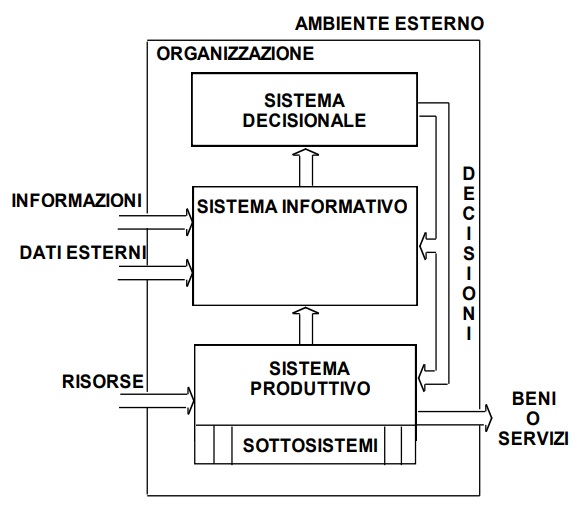
\includegraphics[scale=0.7]{sisinformativoorg.png}
\end{center}
\subsection{Sistemi Informatici}
\paragraph{Sistema Informativo Automatizzato} Quella parte del sistema informativo in cui le informazioni sono raccolte, elaborate, archiviate e scambiate usando un \textbf{sistema informatico}.
\paragraph{Sistema Informatico} Insieme delle tecnologie informatiche e della comunicazione (\textbf{ICT}, Information and Communication Technologies) a supporto delle attività di un'organizzazione.
\paragraph{Terminologia}
\begin{center}
Sistema informativo $\longrightarrow$ Sistema informativo automatizzato\\
Sistema informativo automatizzato $\longrightarrow$ Sistema informatico
\end{center}
\begin{center}
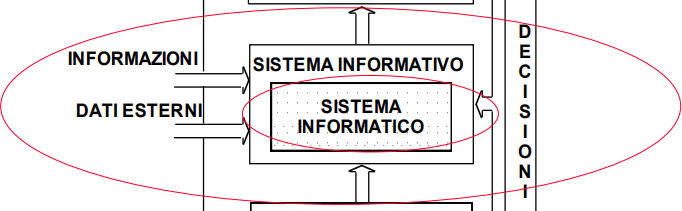
\includegraphics[scale=0.7]{sisinformativoorg2.png}
\end{center}
\pagebreak
\subsection{Classificazione dei sistemi informatici}
\begin{center}
Sistemi Informatici Operativi $\longrightarrow$ Sistemi Informatici Direzionali
\end{center}
\begin{multicols}{2}
\paragraph{Sistemi Informatici Operativi} I dati sono organizzati di DB. Le applicazioni si usano per svolgere le classiche attività strutturate e ripetitive dell'azione nelle aree amministrativa e finanziaria: vendite, risorse umane, produzione\ldots\\
\textbf{Alcune sigle}:
\begin{list}{}{}
	\item \textbf{DP} Data Processing\\\textbf{EDP} Electronic Data Processing
	\item \textbf{TPS} Transaction Processing Systems
\end{list}
\begin{center}
	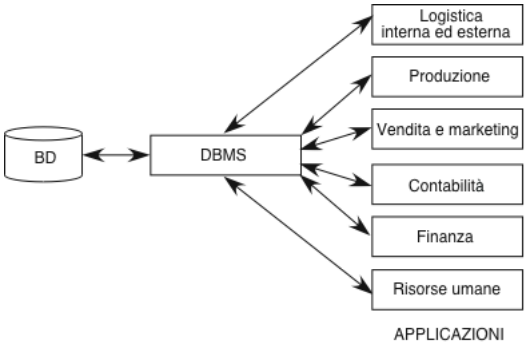
\includegraphics[scale=0.6]{sisinfop.png}
\end{center}
\paragraph{DBMS} Le caratteristiche del DB sono \textbf{garantite da un sistema per la gestione della base di dati} (\textbf{DBMS}, Data Base Management System) che ha il controllo dei dati e li rende accessibili agli utenti autorizzati.
\paragraph{OLTP} \textbf{On-Line Transaction Processing}, modo d'uso principale dei DBMS. Tradizionale elaborazione di transazioni, che realizzano processi operativi per il funzionamento di organizzazioni:
\begin{list}{}{}
	\item Operazioni predefinite e relativamente semplici
	\item Ogni operazione coinvolge \textit{pochi} dati
	\item Dati di dettaglio, aggiornati
\end{list}
\end{multicols}
\begin{multicols}{2}
\paragraph{Sistemi Informatici Direzionali} I dati sono organizzati in data warehouse (DW) e gestiti ad un opportuno sistema. Le applicazioni, dette di \textbf{business intelligence}, sono strumenti di supporto ai processi di controllo delle prestazioni aziendali e di decisione manageriale. Terminologia:
\begin{list}{}{}
	\item \textbf{MIS} Management Information Systems
	\item \textbf{DSS} Decision Support Systems, data-based o model-based
	\item \textbf{EIS} Executive Information System
\end{list}
\begin{center}
	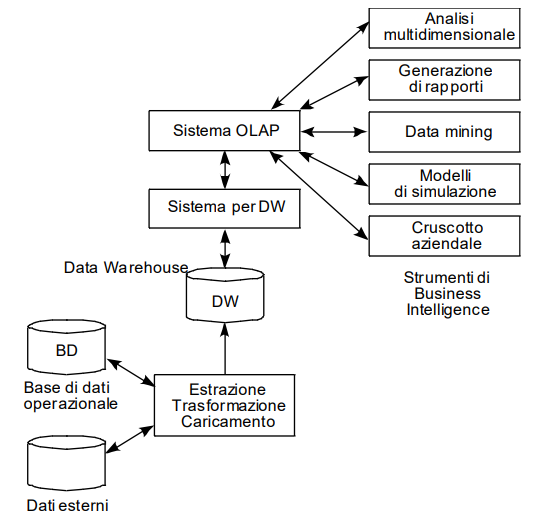
\includegraphics[scale=0.6]{sisinfdir.png}
\end{center}
\columnbreak
\paragraph{OLAP} \textbf{On-Line Analytical Processing} modo d'uso principale dei DW. Analisi dei dati di supporto alle decisioni:
\begin{list}{}{}
	\item Operazioni complesse e casuali
	\item Ogni operazione può coinvolgere \textit{molti} dati
	\item Dati aggregati, storici, anche non attualissimi
\end{list}
\end{multicols}
\pagebreak
\paragraph{Differenze tra OLTP e OLAP}
\begin{center}
	\begin{tabular}{r | l | l}
	 & \makecell{\textbf{OLTP}} & \makecell{\textbf{OLAP}} \\
	\textbf{Scopi} & Supporto operatività & Supporto decisioni \\
	\textbf{Utenti} & Molti, esecutivi & Pochi, dirigenti e analisti \\
	\textbf{Dati} & Analitici, relazionali & Sintetici, multidimensionali \\
	\textbf{Usi} & Noti a priori & Poco prevedibili \\
	\textbf{Quantità di dati per attività} & Bassa (decine) & Alta (milioni) \\
	\textbf{Orientamento} & Applicazione & Soggetto \\
	\textbf{Aggiornamenti} & Frequenti & Rari \\
	\textbf{Visione dei dati} & Corrente & Storica \\
	\textbf{Ottimizzati per} & Transazioni & Analisi
	\end{tabular}
\end{center}
\subsection{Requisiti per l'Analisi dei Dati}
\paragraph{Aggregati} Non interessa \textbf{un} dato, ma la \textbf{somma}, la \textbf{media}, il \textbf{minimo}/\textbf{massimo} di una misura\ldots
\paragraph{Multidimensionale} Interessa \textbf{incrociare le informazioni}, per analizzarle da punti di vista diversi e valutare i risultati del business per intervenire sui problemi critici o per cogliere nuove opportunità
\paragraph{Diversi livelli di dettaglio} Per esempio, una volta scoperto un calo delle vendite in un determinato periodo in una specifica regione, si passa ad un'analisi dettagliata nell'area di interesse per cercare di scoprirne le cause (dimensioni con \textbf{gerarchie})
\subsection{Big Data}
\paragraph{Ampio} Big data è un termine ampio riferito a situazioni in cui l'approccio "schema-first" tipico di DB e DW risulta troppo restrittivo o troppo lento.
\paragraph{3 V} Volume, Varietà, Velocità
\paragraph{} I Big Data sono in genere associati a sistemi NoSQL, machine learning e approcci Data Lake.
\section{DBMS}
Un \textbf{DBMS} è un sistema (\textbf{software}) in grado di \textbf{gestire collezioni di dati} che siano, tra le altre cose:
\begin{list}{}{}
	\item \textbf{Grandi}
	\item \textbf{Persistenti}, con un periodo di vita indipendente dalle singole esecuzioni dei programmi che le utilizzano
	\item \textbf{Condivise}, usate da applicazioni diverse
\end{list}
garantendo \textbf{affidabilità} (resistenza a malfunzionamenti hardware e software-recovery) e \textbf{privacy} (con una disciplina e un controllo degli accessi).\\
Come ogni altro software, un DBMS deve essere \textbf{efficiente} (usare al meglio le risorse di spazio e tempo del sistema) ed \textbf{efficace} (rendere produttive le attività degli utilizzatori).\\
Un DBMS offre opportuni linguaggi per:
\begin{list}{}{}
	\item \textbf{Definire lo schema} di un DB, che va definito prima di creare dati
	\item \textbf{Scegliere le strutture dati} per la memorizzazione
	\item Memorizzare i dati \textbf{rispettando i vincoli} definiti nello schema
	\item Recuperare e modificare i dati, interattivamente (\textbf{query language}, linguaggio di interrogazione) o da programmi
\end{list}
\subsection{Dati}
I dati permanenti contenuti in un DB sono divisi in due categorie:
\begin{list}{}{}
	\item \textbf{Metadati}\\
	Descrivono datti sullo schema dei dati, utenti autorizzati, applicazioni, parametri quantitativi\ldots\\
	I metadati sono descritti da uno schema usando il modello dei dati usato dal DBMS e sono interrogabili con le stesse modalità previste dai dati
	\item \textbf{Dati}\\
	Rappresentazioni di certi fatti conformi alle definizioni dello schema. Hanno le seguenti caratteristiche:
	\begin{list}{}{}
		\item Organizzati in \textbf{insiemi strutturati e omogenei}, fra i quali sono definite delle \textbf{relazioni}. La struttura dei dati e le relazioni sono \textbf{descritte nello schema} usando i meccanismi di astrazione del modello dei dati del DBMS.
		\item Sono \textbf{molti}, sia in assoluto che rispetto ai metadati, e non possono essere gestiti in memoria temporanea
		\item Sono \textbf{accessibili mediante transazioni}, \textbf{unità di lavoro atomiche} che \textbf{non possono avere effetti parziali}
		\item Sono \textbf{protetti} sia \textbf{da accesso da parte di utenti non autorizzati}, sia \textbf{da corruzione dovuta a malfunzionamenti} hardware o software
		\item Sono \textbf{utilizzabili contemporaneamente da utenti diversi}
	\end{list}
\end{list}
Il \textbf{modello relazionale dei dati} è il più diffuso fra i DBMS commerciali. Il \textbf{meccanismo di astrazione} fondamentale è la \textbf{relazione} (\textbf{tabella}), sostanzialmente un insieme di record dai campi elementari.\\
Lo schema di una relazione ne definisce il nome e ne descrive la struttura dei possibili elementi della relazione (insieme di attributi con il loro tipo)
\paragraph{Esempio}
\begin{list}{}{}
	\item \textbf{Definizione del DB}
	\begin{lstlisting}
create database EsempioEsame
	\end{lstlisting}
	\item \textbf{Definizione schema}
	\begin{lstlisting}
create table Esami(Materia char(5), Candidato char(8), Voto int, Lode char(1),
Data char(6))
	\end{lstlisting}
	\item \textbf{Inserzione dati}
	\begin{lstlisting}
insert into Esami values ('BDSI1', '080709', 30 'S', '070900')
	\end{lstlisting}
	\item \textbf{Interrogazione}
	\begin{lstlisting}
select Candidato from Esami where Materia = "BDSI1" and Voto = 30
	> Candidato
	> 080709
	\end{lstlisting}
\end{list}
\pagebreak
\subsection{DDL}
\paragraph{Data Definition Language} Linguaggio per la definizione della base di dati.\\
Utile distinguere tre diversi livelli di descrizione dei dati (\textbf{schemi}):
\begin{multicols}{2}
\begin{list}{}{}
	\item Livello di \textbf{vista logica}
	\item Livello \textbf{logico}
	\item Livello \textbf{fisico}
\end{list}
\begin{center}
	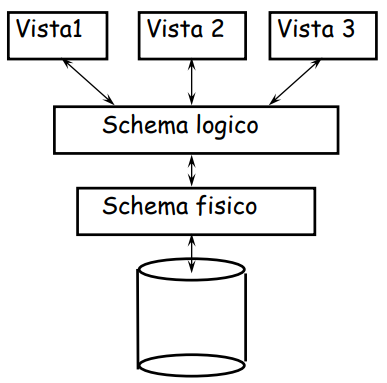
\includegraphics[scale=0.5]{livellidescrdati.png}
\end{center}
\end{multicols}
\paragraph{Livello Logico} Descrive la struttura degli insiemi di dati e delle relazioni fra loro, secondo un erto modello dei dati, senza nessun riferimento alla loro organizzazione fisica nella memoria permanente.\\
Esempi:
\begin{lstlisting}
Studenti(Matricola char(8), Nome char(20), Login char(8), Anno int, Reddito float)
Corsi(IdeC char(8), Titolo char(20), Credito int)
Esami(Matricola char(8), IdeC char(8), Voto int)
\end{lstlisting}
\paragraph{Livello Fisico} Descrive come vanno organizzati fisicamente i dati nelle memorie permanenti e quali strutture dati ausiliarie prevedere per facilitarne l'uso (schema fisico o interno).\\
Esempi: relazioni Studenti e Esami organizzate in modo seriale, Corsi organizzata sequenziale con indice, indice su Matricola.
\paragraph{Vista Logica} Descrive come deve \textbf{apparire la struttura} del DB ad una certa applicazione (\textbf{schema esterno} o \textbf{vista}). Esempio:
\begin{lstlisting}
InfCorsi (IdeC char(8), Titolo char(20), NumEsami int)
\end{lstlisting}
Nell'organizzazione di una banca, lo \textbf{schema logico} conterrà tutte le tabelle e i dati relativi ai conti correnti, ma anche al personale. Lo schema logico conserva \textbf{tutte le informazioni} della banca. Nello \textbf{schema esterno} ogni correntista potrà \textbf{accedere solo ad alcune informazioni} di suo interesse: quelle del proprio conto corrente.
\paragraph{Indipendenza} L'approccio con tre livelli è stato proposto per garantire le proprietà di indipendenza logica e fisica dei dati, fra gli obiettivi più importanti dei DBMS.
\begin{list}{}{}
	\item \textbf{Indipendenza fisica}: i programmi applicativi non devono essere modificati in seguito a modifiche dell'organizzazione fisica dei dati
	\item \textbf{Indipendenza logica}: i programmi applicativi non devono essere modificati in seguito a modifiche dello schema logico
\end{list}
\subsection{DML}
\paragraph{Data Manipulation Language} Linguaggio per l'uso dei dati.\\
Un DBMS deve prevedere più modalità d'uso per soddisfare esigenze di diverse categorie d'utenti: GUI per accedere ai dati, linguaggio di interrogazione per i non programmatori, linguaggio di programmazione per chi sviluppa le applicazioni, linguaggio di sviluppo per le interfacce delle applicazioni.\\
Linguaggi vari e interfacce diverse:
\begin{list}{}{}
	\item Linguaggi testuali interattivi, SQL
	\item Comandi (come quelli del linguaggi interattivo) immersi in un linguaggio ospite, come il C
	\item Comandi (come quelli del linguaggi interattivo) immersi in un linguaggio ad hoc (come PL/SQL) con anche altre funzionalità (come grafici e stampe strutturate)
	\item Interfacce amichevoli
\end{list}
\subsection{Schemi e Istanze}
\paragraph{Schema} Descrive la \textbf{struttura dei dati}, sostanzialmente invariante nel tempo: le "classi", intestazione delle tabelle
\paragraph{Istanza} \textbf{Valori attuali} dei dati che possono cambiare anche molto rapidamente: gli "oggetti", il corpo di ciascuna tabella
\subsection{Meccanismi per il controllo dei dati}
Caratteristica molto importante dei DBMS è il tipo di meccanismi usati per garantire le seguenti proprietà
\begin{list}{}{}
	\item \textbf{Integrità}: mantenimento delle proprietà specificate nello schema
	\item \textbf{Sicurezza}: protezione da usi non autorizzati
	\item \textbf{Affidabilità}: protezione da malfunzionamenti e interferenze dovute all'accesso concorrente di più utenti
\end{list}
\subsection{Transazioni}
\paragraph{Definizione} Una \textbf{transazione} è una \textbf{sequenza di azioni di lettura/scrittura in memoria permanente e di elaborazione dati in memoria temporanea}, con le seguenti proprietà:
\begin{list}{}{}
	\item \textbf{Atomicità}: le transazioni che terminano prematuramente (\textbf{aborted transactions}) sono \textbf{trattate dal sistema come se non fossero mai iniziate}. Eventuali effetti sul DB sono \textbf{annullati}.
	\item \textbf{Serializzabilità}: esecuzioni concorrenti di più transazioni danno come effetto quello di una esecuzione seriale
	\item \textbf{Persistenza}: le \textbf{modifiche} sul DB di una transazione terminata normalmente sono \textbf{permanenti}, cioè \textbf{non alterabili da malfunzionamenti}
\end{list}
\section{Progettazione}
\paragraph{Progettare} Progettare un DB significa \textbf{progettare la struttura dei dati e delle applicazioni}. La progettazione dei dati è l'attività più importante e per progettare al meglio i dati è necessario che essi siano un \textbf{modello fedele del dominio} in esame. Per questo ora parleremo della \textbf{modellazione}.
\subsection{Modellazione}
\paragraph{Definizione} Un \textbf{modello astratto} è la \textbf{rappresentazione formale di idee e conoscenze relative ad un fenomeno}.\\
Aspetti di un modello:
\begin{list}{}{}
	\item Il \textbf{modello} è la \textbf{rappresentazione di certi fatti}.
	\item La \textbf{rappresentazione} è \textbf{data con un linguaggio formale}.
	\item Il \textbf{modello} è \textbf{il risultato di un processo di interpretazione}, guidato dalle idee e conoscenze possedute dal soggetto che interpreta.
\end{list}
\textbf{La stessa realtà può utilmente essere modellata in modi diversi e a diversi livelli di astrazione}.
\begin{center}
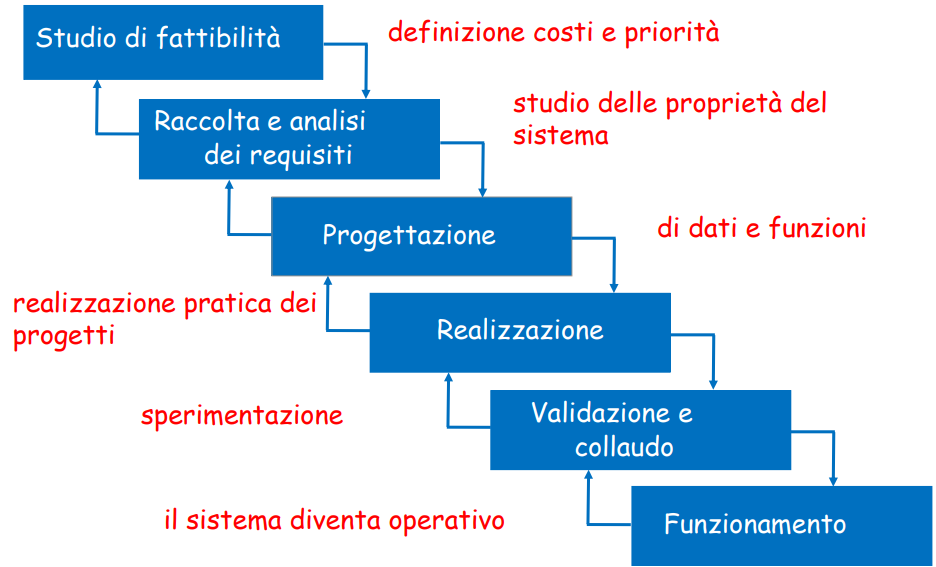
\includegraphics[scale=0.7]{modellaz.png}
\end{center}
\paragraph{Metodologia di progetto} Per garantire prodotti di buona qualità è opportuno seguire una metodologia di progetto, con:
\begin{list}{}{}
	\item Articolazione delle attività in fasi (\textbf{decomposizione})
	\item Criteri di scelta (\textbf{strategie})
	\item \textbf{Modelli} da rappresentare
	\item \textbf{Generalità} rispetto al problema in esame e agli strumenti a disposizione
	\item \textbf{Qualità} del prodotto
	\item \textbf{Facilità d'uso}
\end{list}
\paragraph{Progettazione della base di dati} Suddivisa nelle seguenti fasi:
\begin{enumerate}
	\item \textbf{Analisi} dei requisiti
	\item Progettazione \textbf{concettuale}
	\item Progettazione \textbf{logica}
	\item Progettazione \textbf{fisica}
\end{enumerate}
Ciascuna fase è incentrata sulla modellazione, che discuteremo quindi con riferimento alla problematica della progettazione del DB.
\paragraph{Modello dei dati} Insieme di costrutti utilizzati per organizzare i dati di interesse e descriverne la dinamica. Il componente fondamentale è l'insieme dei \textbf{meccanismi di strutturazione} (o \textbf{costruttori di tipo}). Come nei linguaggi di programmazione, esistono meccanismi che permettono di definire nuovi tipi, così \textbf{ogni modello dei dati prevede alcuni costruttori}: per esempio, il \textbf{modello relazionale prevede il costruttore \textit{relazione}}, che permette di definire insiemi di record omogenei.
\pagebreak
\subsection{Aspetti del problema}
\subsubsection{Aspetto ontologico} Quale conoscenza del dominio del discorso si rappresenta? Ontologico cioè studio di ciò che si suppone esista nell'universo del discorso e che sia quindi necessario modellare.
\begin{list}{}{Cosa si modella:}
	\item \textbf{Conoscenza concreta}: i fatti
	\item \textbf{Conoscenza astratta}: la struttura e i vincoli sulla conoscenza concreta
	\item \textbf{Conoscenza procedurale}, comunicazioni: le operazioni base, le operazioni degli utenti, come si comunicherà con il sistema informatico
\end{list}
Ci concentreremo sulla conoscenza concreta e astratta.
\subsubsection{Aspetto logico} Con quali meccanismi di astrazione si modella? Il modello dei dati a oggetti.
\paragraph{Modello dei dati} Insieme dei meccanismi di astrazione per descrivere la struttura della conoscenza concreta.\\
\textbf{Schema}: descrizione della \textbf{struttura della conoscenza concreta} e dei \textbf{vincoli di integrità} usando un particolare modello dei dati.\\\\
Useremo come notazione grafica una \textbf{variante} dei diagrammi a oggetti (o diagrammi Entità-Relazione, diagrammi ER). Nozioni fondamentali: oggetto, tipo di oggetto, classe, ereditarietà, gerarchia fra tipi e gerarchia fra classi.
\subsubsection{Aspetto linguistico} Con quale linguaggio formale si definisce un modello?
\subsubsection{Aspetto pragmatico} Come si procede per costruire un modello? Metodologia da seguire nel processo di modellazione, cioè l'insieme di regole finalizzate alla costruzione del modello informatico.
\subsection{Conoscenza concreta}
La conoscenza concreta riguarda i fatti specifici che si vogliono rappresentare:
\begin{list}{}{}
	\item \textbf{Entità}, sono \textbf{ciò di cui interessa rappresentare alcuni fatti o proprietà}. Ad esempio: una descrizione bibliografica di un libro, un libro, un documento, un prestito, un utente della biblioteca\ldots\\
	Le \textbf{proprietà} sono \textbf{fatti che interessano solo in quanto descrivono caratteristiche di determinate entità}. Ad esempio un indirizzo interessa perché è l'indirizzo di un utente. Hanno delle classificazioni:
	\begin{list}{}{}
		\item Primitiva/strutturata
		\item Obbligatoria/opzionale
		\item Univoca/multivalore
		\item Costante/variabile
		\item Calcolata/non calcolata
	\end{list}
	Una proprietà è una coppia attributo-valore di un certo tipo. Ogni entità appartiene ad un \textbf{tipo} che ne specifica la natura. Ogni proprietà ha associato un \textbf{dominio}, l'insieme dei possibili valori.\\
	Una proprietà è \textbf{atomica} se il suo valore non è scomponibile, altrimenti è \textbf{strutturata}. Inoltre è \textbf{univoca} se ha valore unico, altrimenti è \textbf{multivalore}, e \textbf{totale} (obbligatoria) se ogni entità dell'universo in esame ha per essa un valore specificato, altrimenti è detta \textbf{parziale} (opzionale)\\\\
	Certi fatti possono essere interpretati come proprietà in certi contesti e come entità in altri. Ad esempio, una \texttt{DescrizioniBibliografiche} con attributi \texttt{autori}, \texttt{titolo}, \texttt{editore}\ldots, \textbf{oppure} un \texttt{Autori} con attributi \texttt{nome}, \texttt{nazionalità}\ldots e \texttt{Editori} con \texttt{nome}, \texttt{indirizzo}\ldots
	\item \textbf{Collezioni} variabili nel tempo di entità omogenee. Ad esempio, la collezione di tutti gli utenti della biblioteca.
	\item \textbf{Associazioni} fra entità
\end{list}
\subsection{Modellazione ad oggetti}
\paragraph{Oggetti} Ad ogni entità del dominio corrisponde un oggetto del modello. Un \textbf{oggetto} è un'\textbf{entità software con stato, comportamento ed identità} che modella un'entità dell'universo.
\begin{list}{}{}
	\item \textbf{Stato} modellato da un insieme di costanti o variabili con valori di qualsiasi complessità
	\item \textbf{Comportamento} dato da un insieme di procedure locali chiamate \textbf{metodi}, che modellano le operazioni di base che riguardano l'oggetto e le proprietà derivabili da altre.
	\item Un oggetto può rispondere a dai \textbf{messaggi}, restituendo valori memorizzati nello stato o calcolati con una procedura locale.
\end{list}
\paragraph{Classe} \textbf{Insieme di oggetti dello stesso tipo}, modificabile con operatori per includere o estrarre elementi dall'insieme. Può essere specificata a diversi livelli.
\begin{center}
	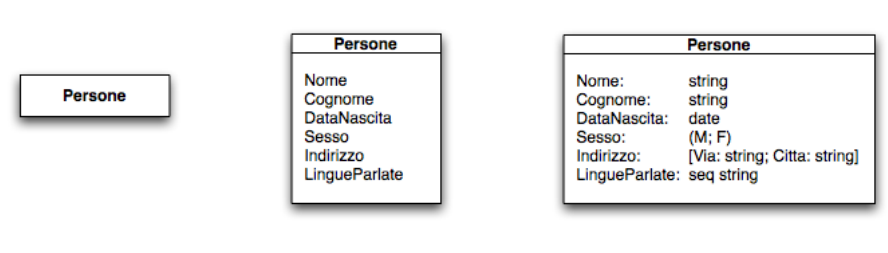
\includegraphics[scale=0.75]{classspec.png}
\end{center}
\paragraph{Tipo oggetto} Il primo passo nella costruzione di un modello consiste nella classificazione delle entità del dominio con la definizione dei tipi degli oggetti che la rappresentano.\\
Un \textbf{tipo oggetto definisce l'insieme dei messaggi} (\textbf{interfaccia}) \textbf{a cui può rispondere un insieme di possibili oggetti}. I nomi dei messaggi sono detti anche attributi degli oggetti.\\
Nei diagrammi ER i tipi oggetti non si rappresentano, perché l'attenzione è sulle collezioni e sulle associazioni. Tuttavia, la rappresentazione grafica di una collezione indica anche gli attributi del tipo oggetto associato.
\paragraph{Associazioni} Un'\textbf{istanza di associazione} è un \textbf{fatto che correla due o più entità}, stabilendo un legame  logico fra loro. Ad esempio, l'utente Tizio ha in prestito una copia della Divina Commedia.\\
Un'associazione \texttt{R(X, Y)} fra due collezioni di entità \texttt{X} e \texttt{Y} è un \textbf{insieme di istanze di associazione} tra elementi di \texttt{X} e di \texttt{Y} che \textbf{varia in generale nel tempo}.\\
Il prodotto cartesiano \texttt{X $\times$ Y} è il dominio dell'associazione.\\
Un esempio:
\begin{center}
	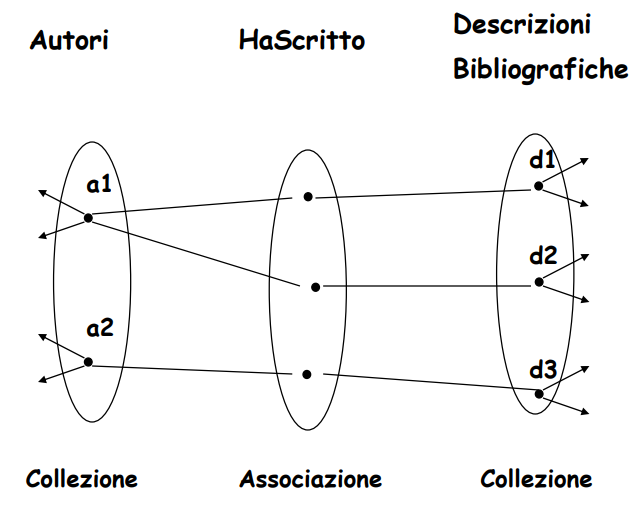
\includegraphics[scale=0.6]{associazioni.png}
\end{center}
\pagebreak
Un associazione è \textbf{caratterizzata da due proprietà strutturali}: \textbf{molteplicità} e \textbf{totalità}.
\subparagraph{Vincolo di univocità} Un'associazione \texttt{R(X, Y)} è \textbf{univoca rispetto a \texttt{X}} se $\forall$\texttt{x} $\in$ \texttt{X} $\exists$ al più un elemento di \texttt{Y} associato ad \texttt{x}.\\
Se non vale questo vincolo, l'associazione è \textbf{multivalore rispetto ad \texttt{X}}.\\\\
\textbf{Cardinalità} dell'associazione:
\begin{list}{}{}
	\item \texttt{R(X, Y)} è \texttt{1:N} se è multivalore su \texttt{X} ed univoca su \texttt{Y}
	\item \texttt{R(X, Y)} è \texttt{N:1} se è univoca su \texttt{X} e multivalore su \texttt{Y}
	\item \texttt{R(X, Y)} è \texttt{N:M} se è multivalore su \texttt{X} e multivalore  su \texttt{Y}
	\item \texttt{R(X, Y)} è \texttt{1:1} se è univoca su \texttt{X} ed univoca su \texttt{Y}
\end{list}
Qualche esempio:
\begin{list}{}{}
	\item \texttt{Frequenta(Studenti, Corsi)} ha cardinalità \texttt{N:M}
	\item \texttt{Insegna(Professori, Corsi)} ha cardinalità \texttt{1:N}
	\item \texttt{SuperatoDa(Esami, Studenti)} ha cardinalità \texttt{N:1}
	\item \texttt{Dirige(Professori, Dipartimenti)} ha cardinalità \texttt{1:1}
\end{list}
\subparagraph{Vincolo di totalità} Un associazione \texttt{R(X, Y)} è \textbf{totale} (o surgettiva) su \texttt{X} se $\forall$ \texttt{x} $\in$ \texttt{X} $\exists$ almeno un elemento di \texttt{Y} associato ad \texttt{x}.\\
Se non vale questo vincolo, l'associazione è \textbf{parziale rispetto a \texttt{X}}.\\
Ad esempio, \texttt{Insegna(Professori, Corsi)} è totale su \texttt{Corsi} perché non può esistere un corso senza il corrispondente docente.
\paragraph{Rappresentazione} Un'associazione si rappresenta con una linea che collega le classi che rappresentano le due collezioni. La linea è etichettata con il nome dell'associazione, di solito scelto utilizzando un predicato.\\
L'univocità dell'associazione rispetto ad una classe si rappresenta disegnando una freccia singola sulla linea che esce dalla classe ed entra nella destinazione. L'assenza di tale vincolo è indicata da una freccia doppia.\\
Similmente, la parzialità è rappresentata da un taglio vicino alla freccia, mentre la totalità è rappresentata dall'assenza del taglio.
\begin{center}
	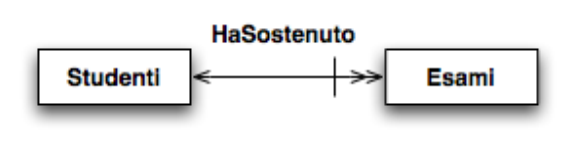
\includegraphics[scale=0.5]{assocesemp.png}\\
	Ogni esame riguarda uno ed un solo studente\\
	Parzialità e assenza di univocità sugli esami\\
	superati da uno studente.\\
	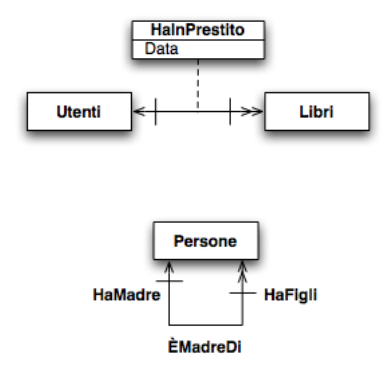
\includegraphics[scale=0.65]{assocesemp2.png}\\
	Possono avere proprietà ed essere ricorsive.
\end{center}
\pagebreak
\subsection{Sottoclassi}
\begin{center}
	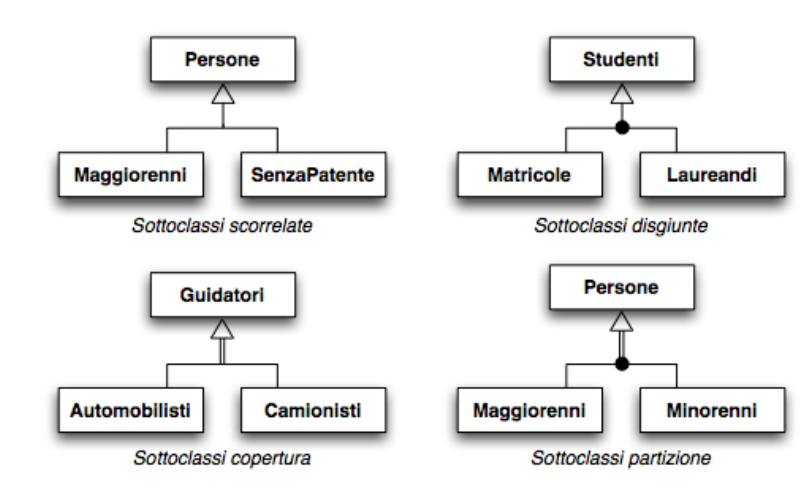
\includegraphics[scale=0.5]{sottoclassi.png}
\end{center}
\paragraph{Vincoli}
\begin{list}{}{}
	\item \textbf{Vincolo intensionale}: C sottoclasse di C' $\Rightarrow$ tipo degli elementi di C è sottotipo del tipo degli elementi di C'
	\item \textbf{Vincolo estensionale}: C sottoclasse di C' $\Rightarrow$ gli elementi di C sono un sottoinsieme degli elementi di C'
	\item \textbf{Disgiunzione}: ogni coppia di sottoclassi è disgiunta, priva di elementi comuni (pallino nero) \textbf{sottoclassi disgiunte})
	\item \textbf{Copertura}: l'unione degli elementi delle sottoclassi coincide con l'insieme degli elementi della superclasse (freccia con doppia asta) (\textbf{sottoclassi copertura})
\end{list}
\subsection{Un esempio elaborato}
\begin{center}
	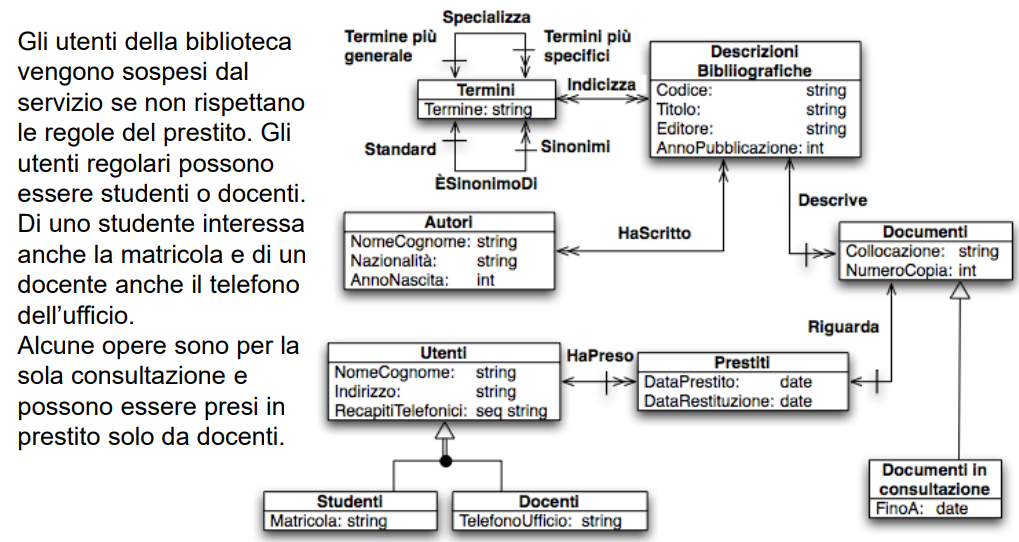
\includegraphics[scale=0.65]{esempioelaborato.png}
\end{center}
\pagebreak
\subsection{Conoscenza astratta}
La conoscenza astratta riguarda i \textbf{fatti generali che descrivono}
\begin{list}{}{}
	\item la \textbf{struttura della conoscenza concreta}, come collezioni, tipi entità, associazioni\ldots
	\item le \textbf{restrizioni sui valori} possibili della conoscenza concreta e sui modi in cui essi possono evolvere nel tempo (\textbf{vincoli d'integrità}, statici e dinamici)
	\item le \textbf{regole per derivare fatti nuovi} da altri noti
\end{list}
\paragraph{Vincoli} Possono essere descritti in \textbf{modo dichiarativo} (da preferire), con formule di calcolo dei predicati, oppure mediante controlli da eseguire nelle operazioni.
\begin{center}
	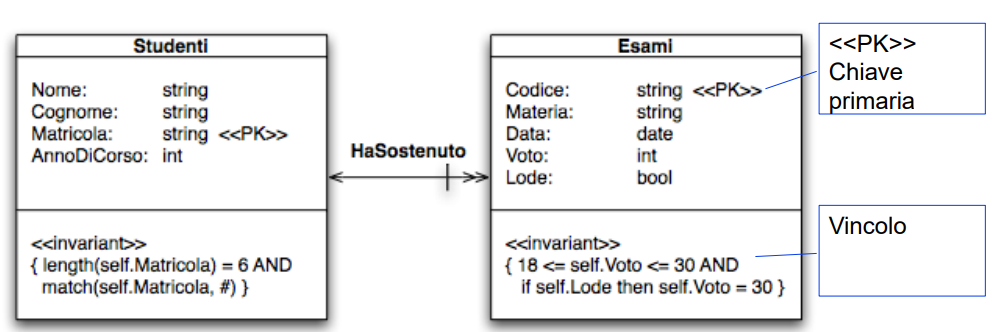
\includegraphics[scale=0.6]{vincoli.png}
\end{center}
\section{Costruzione}
\begin{enumerate}
	\item Analisi dei requisiti $\rightarrow$ specifica dei requisiti, schemi di settore
	\item Progettazione
	\begin{list}{-}{}
		\item Progettazione \textbf{concettuale} ($\rightarrow$ schema concettuale), \textbf{logica} ($\rightarrow$ schema logico), \textbf{fisica} ($\rightarrow$ schema fisico) dei dati
		\item Progettazione delle applicazioni
	\end{list}
	\item Realizzazione
\end{enumerate}
Spesso consideriamo l'analisi dei requisiti come parte della progettazione.
\subsection{Analisi dei requisiti}
\textbf{Analizza il sistema} esistente e \textbf{raccoglie requisiti informali}. Dopodiché \textbf{elimina le ambiguità} e la disuniformità, \textbf{raggruppando frasi relative a diverse categorie} di dati, vincoli e operazioni.\\
Costruisce un \textbf{glossario}, \textbf{disegna lo schema} di settore, \textbf{specifica le operazioni} e \textbf{verifica la coerenza tra operazioni e dati}.
\paragraph{Documentazione descrittiva} In generale, il linguaggio naturale è pieno di ambiguità e fraintendimenti, che bisogna evitare per quanto possibile. Come prima approssimazione si può seguire queste regole:
\begin{list}{}{}
	\item Studiare e comprendere il sistema informativo ed i bisogni informativi di tutti i settori dell'organizzazione
	\item \textbf{Scegliere} il corretto \textbf{livello di astrazione}
	\item \textbf{Standardizzare la scrittura delle frasi}
	\item \textbf{Suddividere le frasi} articolate
	\item \textbf{Separare} le frasi sui \textbf{dati} da quelle sulle \textbf{funzioni}
\end{list}
\paragraph{Organizzare i concetti e i termini} Regole generali
\begin{list}{}{}
	\item Eliminare le ambiguità, le imprecisioni e la disuniformità: individuare omonimi e sinonimi e unificare i termini
	\item Riorganizzare le frasi per \textbf{concetti}, ovvero ottenendo diverse categorie di dati, vincoli e operazioni
	\item Costruire un \textbf{glossario} dei termini
	\item Disegnare lo schema
	\item Specificare le operazioni
	\item Verificare la coerenza fra le operazioni e i dati
\end{list}
\end{document}